
\subsection{Binomische Formeln}
Im Folgenden werden wir häufig besonders einfache Terme antreffen: die sogenannten Polynome.

\begin{definition}{Polynome}{polynome}
    \textbf{Polynome} sind Terme, in denen Vielfache der Variablen miteinander addiert und multipliziert werden.
\end{definition}

\textbf{Beispiele:}
\[
    3xy^3
\]
\[
    2a+3b^2
\]

Die Zahlen, mit denen die Variablen multipliziert werden, heissen \textbf{Koeffizienten}. Das zweite Beispiel besteht aus zwei Summanden und heisst deswegen \textbf{Binom}. Das erste Beispiel besteht nur aus einem Summanden und wird \textbf{Monom} genannt. Wenn es drei Summanden sind, wird der Term \textbf{Trinom} genannt. Und schliesslich wird ein Term, der aus mehreren Summanden besteht, eben \textbf{Polynom} genannt. (griechisch \enquote{polys} = \enquote{viel})

Manchmal sieht man den Termen nicht gleich an, ob sie Polynome sind. So ist \((a+b)^3\) auch ein Polynom, denn durch Ausmultiplizieren erhält man (mit einigen Zwischenschritten)
\[
    (a+b)^3=a^3+3a^2b+3ab^2+b^3.
\]

Diese einfachste Darstellung eines Polynoms als Summe von Monomen heisst \textit{Normalform}.

Zum Schluss noch Beispiele für Terme, die keine Polynome sind:
\[
    \frac{1}{a},
    \qquad
    3^x,
    \qquad
    \sqrt{a+b}.
\]

\begin{LA}
    {Binomische Formeln}{binomische-formeln}
    \begin{enumerate}
        \item Vereinfachen Sie den Term
              \[
                  (a+b)^2=(a+b)(a+b),
              \]
              indem Sie \enquote{jede mit jeder} ausmultiplizieren und das Resultat vereinfachen. Fügen Sie das Resultat in den folgenden Kasten ein:

              \begin{center}
                  \fbox{
                      \begin{minipage}{0.85\textwidth}
                          \textbf{Erste Binomische Formel:}
                          \[
                              (a+b)^2= \phantom{a^2+2ab+b^2}
                          \]
                          \vspace*{0.25cm}

                      \end{minipage}
                  }
              \end{center}
              %   \clearpage

        \item Nutzen Sie die erste Binomische Formel, um die folgenden Quadrate \textbf{ohne \enquote{jede mit jeder}} zu berechnen:

              \begin{enumerate}
                  \item \((x+y)^2\)\vspace*{0.5cm}
                  \item \((x+3)^2\)\vspace*{0.5cm}
                  \item \((q+2p)^2\)\vspace*{0.5cm}
                  \item \((x+y^3)^2\)\vspace*{0.5cm}
              \end{enumerate}

        \item Finden Sie auch die zweite und dritte binomische Formel, indem Sie \enquote{jede mit jeder} rechnen. Füllen Sie den Kasten aus.

              \begin{center}
                  \fbox{
                      \begin{minipage}{0.85\textwidth}
                          \textbf{Zweite Binomische Formel:}
                          \[
                              (a-b)^2=\phantom{a^2-2ab+b^2}
                          \]

                          \textbf{Dritte Binomische Formel:}
                          \[
                              (a+b)(a-b)=\phantom{a^2-b^2}
                          \]
                          \vspace*{0.25cm}
                      \end{minipage}
                  }
              \end{center}


        \item Nutzen Sie die drei Binomischen Formeln, um die folgenden Produkte
              \textbf{ohne \enquote{jede mit jeder}} zu berechnen:

              \begin{enumerate}
                  \item \((2x+y)(2x-y)\) \vspace*{0.5cm}
                  \item \((x-6)^2\) \vspace*{0.5cm}
                  \item \((x-3y)^2\) \vspace*{0.5cm}
                  \item \((x^4+y)(x^4-y)\) \vspace*{0.5cm}
              \end{enumerate}

        \item Die Babylonier sind ein Volk, das in Mesopotamien, einer fruchtbaren Ebene zwischen den Flüssen Euphrat und Tigris, im heutigen Irak lebte. Sie entwickelten eine Schrift, die aus keilförmigen Symbolen bestand und mit Stiften in Tonplatten gedrückt wurde. Anschliessend wurden die Platten in der Sonne getrocknet. Viele Tausende dieser Tafeln existieren noch heute. Das folgende Bild zeigt die Zahlen von \(1\) bis \(59\) in Keilschrift:

              \begin{center}
                  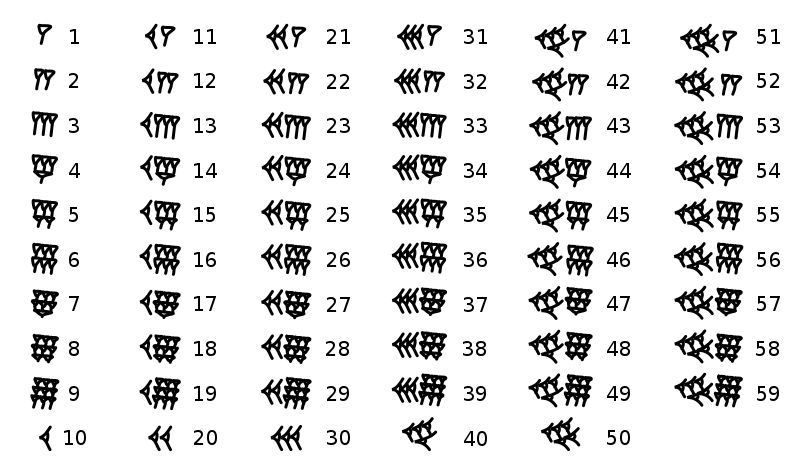
\includegraphics[width = 0.5 \textwidth]{media/babylonische_ziffern-320401102.png}
              \end{center}

              Unter den Keilschrift-Tafeln wurden einige gefunden, welche die Quadratzahlen
              \[
                  1,4,9,16,25,36,\ldots
              \]
              aufgelistet haben. Lange wurde darüber gerätselt, zu welchem Zweck diese Listen angefertigt wurden. Dann hat man herausgefunden, dass die Babylonier diese Listen dazu verwendeten, um beliebige Zahlen miteinander zu multiplizieren:

              Sollten die Zahlen \(a\) und \(b\) miteinander multipliziert werden, bildeten sie zunächst die Summe \((a+b)\) und die Differenz \((a-b)\), ermittelten dann die Quadrate der Summe und der Differenz mit Hilfe der Tafeln und subtrahierten anschliessend die beiden Zahlen voneinander. Schliesslich teilten sie das Ergebnis durch \(4\) und heraus kam das Produkt der beiden Zahlen \(a\) und \(b\).

              \begin{enumerate}
                  \item Berechnen Sie mit diesem Verfahren \(53\cdot47\).

                  \item Erstellen Sie einen Term für das Rechenverfahren der Babylonier und zeigen Sie, dass dieser Term tatsächlich gleich dem Produkt \(a\cdot b\) ist. (Nutzen Sie die binomischen Formeln.)

                  \item Welcher Zusammenhang besteht zwischen dem beschriebenen Rechenverfahren und der Grafik? Tipp: Berechnen Sie die Fläche des grossen Quadrates auf zwei Arten.

                        \begin{center}
                            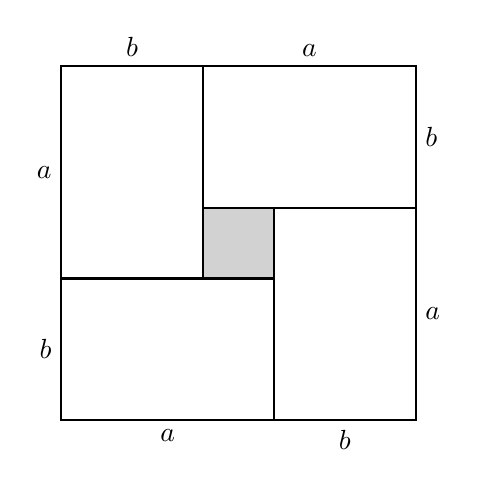
\begin{tikzpicture}[scale=0.9]
                                % Äusseres Quadrat
                                \draw[thick] (0,0) rectangle (5,5);

                                % Innere Unterteilung
                                \draw[thick] (2,5) -- (2,2);
                                \draw[thick] (2,3) -- (5,3);
                                \draw[thick] (3,0) -- (3,3);
                                \draw[thick] (0,2) -- (3,2);

                                % Zentrales Quadrat
                                \fill[gray!35] (2,2) rectangle (3,3);
                                \draw[thick] (2,2) rectangle (3,3);

                                % Beschriftung oben
                                \node[above] at (1,5) {\(b\)};
                                \node[above] at (3.5,5) {\(a\)};

                                % Beschriftung rechts
                                \node[right] at (5,4) {\(b\)};
                                \node[right] at (5,1.5) {\(a\)};

                                % Beschriftung unten
                                \node[below] at (1.5,0) {\(a\)};
                                \node[below] at (4,0) {\(b\)};

                                % Beschriftung links
                                \node[left] at (0,3.5) {\(a\)};
                                \node[left] at (0,1) {\(b\)};
                            \end{tikzpicture}
                        \end{center}

                  \item Finden Sie eine andere Möglichkeit, wie man mit diesen Tafeln multiplizieren kann?
              \end{enumerate}
    \end{enumerate}
\end{LA}






\clearpage
\begin{satz}{Die Binomischen Formeln}{binomischeformeln}
    Für \(a,b\in\mathbb{R}\) gilt:
    \begin{enumerate}
        \item
              \[
                  (a+b)^2=a^2+2ab+b^2
              \]

        \item
              \[
                  (a-b)^2=a^2-2ab+b^2
              \]

        \item
              \[
                  (a+b)(a-b)=a^2-b^2
              \]
    \end{enumerate}
\end{satz}

\textbf{Beweis:}
Zum Beweis muss man bloss die linke Seite ausmultiplizieren. Für die erste Binomische Formel sähe das so aus:
\[
    (a+b)^2
    =(a+b)(a+b)
    =a^2+ab+ba+b^2
    =a^2+2ab+b^2.
\]
Die anderen Formeln können genau gleich bewiesen werden.

\begin{bsp}{Binomische Formeln}{binomischeformeln-bsp}
    Berechnen Sie mithilfe der Binomischen Formeln.
    \begin{enumerate}
        \item \((x+2y)^2\)
              \vspace*{2cm}
        \item \((-p+q)^2\)
              \vspace*{2cm}
        \item \((x^3+y)^2\)
              \vspace*{2cm}
        \item \((-a-b)^2\)
              \vspace*{2cm}
    \end{enumerate}
\end{bsp}


\clearpage
\begin{ueb}
    {Binomische Formeln}{binome}
    \begin{enumerate}
        \item
              \begin{enumerate}
                  \item \((2a+5)^2\)
                  \item \((1-7u)^2\)
                  \item \(\left(\frac{1}{3}a+b\right)^2\)
                  \item \((2n-m)(2n+m)\)
                  \item \((x^2+2)^2\)
                  \item \((4a-5b)^2\)
                  \item \(\left(\frac{1}{4}d-\frac{c}{2}\right)^2\)
                  \item \(\left(\frac{1}{2}x+y\right)\left(\frac{1}{2}x-y\right)\)
              \end{enumerate}

        \item
              \begin{enumerate}
                  \item \(\left(\frac{1}{a}-\frac{1}{b}\right)
                        \left(\frac{1}{b}+\frac{1}{a}\right)\)
                  \item \(\left(\frac{3}{4}a-1\right)^2\)
                  \item \((4x^2+9y^2)^2\)
                  \item \((x^2-1)(x^2+1)\)
                  \item \((-5y+x)^2\)
                  \item \((-x-y)(x+y)\)
                  \item \((-x-y)(x-y)\)
                  \item \((-a-3b)^2\)
              \end{enumerate}
        \item
              \begin{enumerate}
                  \item \(\left(x+\frac{1}{2}\right)\left(\frac{1}{2}-x\right)\)
                  \item \((2e-3f)(3f+2e)\)
                  \item \(2n(7p-6q+1)\)
                  \item \(a(a^2-2b)^2\)
                  \item \((-1)\cdot(2x-3y^2+2xy)\)
                  \item \(2c(c-5)^2\)
              \end{enumerate}

        \item
              \begin{enumerate}
                  \item \((3-y)^2(3+y)^2\)
                  \item \((a+b)^2\cdot\frac{1}{b}\)
                  \item \(\frac{1}{2}x\cdot(y+4)^2\)
                  \item \(\bigl[(2a+b)(2a-b)\bigr]^2\)
                  \item \(\frac{1}{x}\cdot(x+x^2)^2\)
                  \item \((a+4)^2-(a-2)^2\)
                  \item \((2x-y)^2+(2x+y)^2\)
                  \item \((2y+2z)^2-2(y+z)^2\)
                  \item \((5u-1)^2-(5u-1)(5u+1)\)
              \end{enumerate}
    \end{enumerate}
\end{ueb}

\clearpage
\emph{Lösungen}
\begin{enumerate}
    \item
          \begin{enumerate}
              \item \(4a^2+20a+25\)
              \item \(49u^2-14u+1\)
              \item \(\dfrac{1}{9}a^2+\dfrac{2}{3}ab+b^2\)
              \item \(4n^2-m^2\)
              \item \(x^4+4x^2+4\)
              \item \(16a^2-40ab+25b^2\)
              \item \(\dfrac{1}{16}d^2-\dfrac{1}{4}cd+\dfrac{1}{4}c^2\)
              \item \(\dfrac{1}{4}x^2-y^2\)
          \end{enumerate}

    \item
          \begin{enumerate}
              \item \(\dfrac{1}{a^2}-\dfrac{1}{b^2}\)
              \item \(\dfrac{9}{16}a^2-\dfrac{3}{2}a+1\)
              \item \(16x^4+72x^2y^2+81y^4\)
              \item \(x^4-1\)
              \item \(x^2-10xy+25y^2\)
              \item \(-x^2-2xy-y^2\)
              \item \(-x^2+y^2\)
              \item \(a^2+6ab+9b^2\)
          \end{enumerate}

    \item
          \begin{enumerate}
              \item \(\dfrac{1}{4}-x^2\)
              \item \(4e^2-9f^2\)
              \item \(14np-12nq+2n\)
              \item \(a^5-4a^3b+4ab^2\)
              \item \(-2x+3y^2-2xy\)
              \item \(2c^3-20c^2+50c\)
          \end{enumerate}

    \item
          \begin{enumerate}
              \item \(y^4-18y^2+81\)
              \item \(\dfrac{a^2}{b}+2a+b\)
              \item \(\dfrac{1}{2}xy^2+4xy+8x\)
              \item \(16a^4-8a^2b^2+b^4\)
              \item \(x^3+2x^2+x\)
              \item \(12a+12\)
              \item \(8x^2+2y^2\)
              \item \(2y^2+4yz+2z^2\)
              \item \(2-10u\)
          \end{enumerate}
\end{enumerate}






















